\subsection{Optimization}
\label{sec:optimization}

A more stringent selection must be applied on top of the pre-selection
in \sec\ref{sec:preselection_yield} in order to obtain any
sensitivity to the signal.  The best selection, however, is
not known \emph{a priori}. We attempted to find the best possible selection
by starting from a list of kinematic quantities, chosen based on heuristic
arguments. These kinematic quantities, along with the signal
plus background model, are passed into an optimization 
framework that systematically seeks to simultaneously 
maximize the predicted signal and the precision on the final measurement.

The optimization framework considers several thousand
independent permutations of the different
kinematic quantities, along with variations of the selection thresholds
on these cuts, to form combinations of selection cuts which could become a final
selection. 
Each combination is referred to as a separate operating point.
For each operating point
that is considered, the signal plus background
model is evaluated to determine the expected yields and systematic
uncertainties given that selection.  The LHC data is not used in the optimization.  
The prediction is then plugged into the statistical framework described in
\sec\ref{sec:measurement} to extract a value on the expected precision
of the measurement. For each operating point,
the value of the precision is compared against the expected signal yield.
With some discretion, we then choose the operating point 
that maximizes the signal yield and gives the smallest absolute 
precision on the measurement. 
%The shape of the optimization can be seen in \fig\ref{fig:optimization}.


%\begin{figure}[ht!]
%\centering
%
\includegraphics[width=0.3\textwidth]{figures/placeholder.eps}
%
\includegraphics[width=0.3\textwidth]{figures/placeholder.eps}
%
\includegraphics[width=0.3\textwidth]{figures/placeholder.eps}
%\caption{Signal Yield vs Measurement Uncertainty for optimized points 
%in the 0 SFOS (left), 1 SFOS (middle), and 2 SFOS (right) signal regions.}
%\label{fig:optimization}
%\end{figure}

\begin{figure}[htb!]
\centering
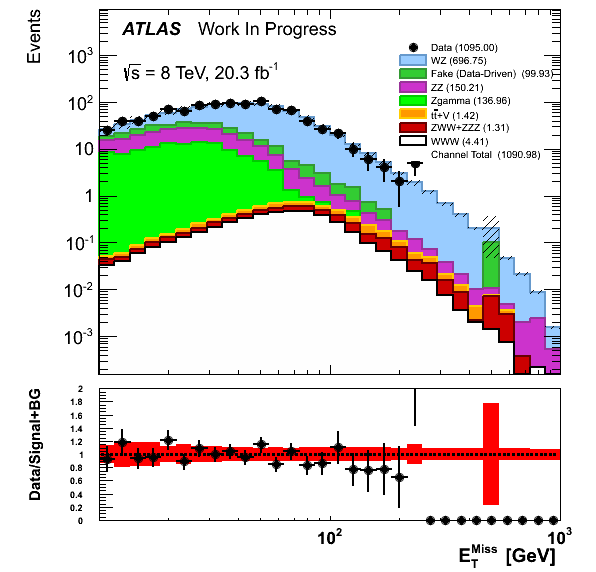
\includegraphics[width=0.495\textwidth]{figures/appendix_signal_selection/Nov24Update_FakeSys_KFacSys_LogY_NoRebin/output/jobs/MxM/DataFull_Rates_May13_FakeRatesExactly2Loose_MuonMxMBJetGt0_ElBJetGt0SubtractPC_MxM/PreselectionNov23_15_1SFOS_ChargeAbs1_BVeto85_physics/weight_all/png/MET_Et_histratio.png}
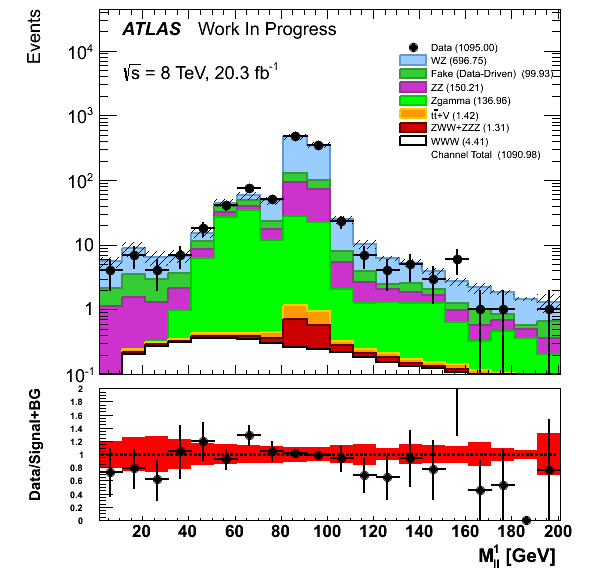
\includegraphics[width=0.495\textwidth]{figures/appendix_signal_selection/Nov24Update_FakeSys_KFacSys_LogY_NoRebin/output/jobs/MxM/DataFull_Rates_May13_FakeRatesExactly2Loose_MuonMxMBJetGt0_ElBJetGt0SubtractPC_MxM/PreselectionNov23_15_1SFOS_ChargeAbs1_BVeto85_physics/weight_all/png/InvariantMassSFOS_histratio.png}
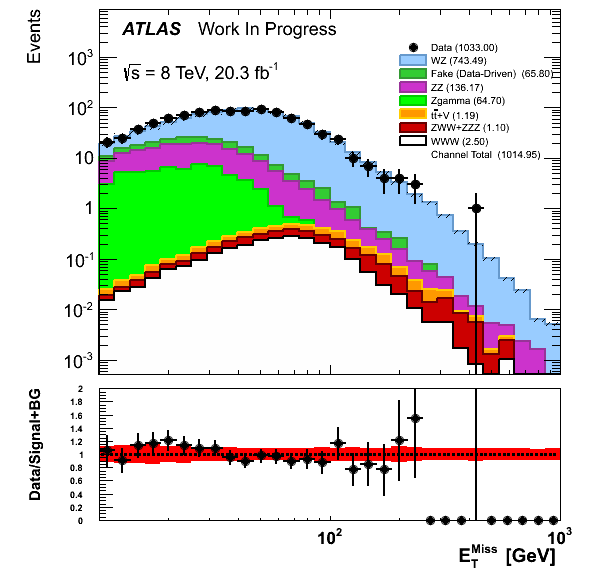
\includegraphics[width=0.495\textwidth]{figures/appendix_signal_selection/Nov24Update_FakeSys_KFacSys_LogY_NoRebin/output/jobs/MxM/DataFull_Rates_May13_FakeRatesExactly2Loose_MuonMxMBJetGt0_ElBJetGt0SubtractPC_MxM/PreselectionNov23_15_2SFOS_ChargeAbs1_BVeto85_physics/weight_all/png/MET_Et_histratio.png}
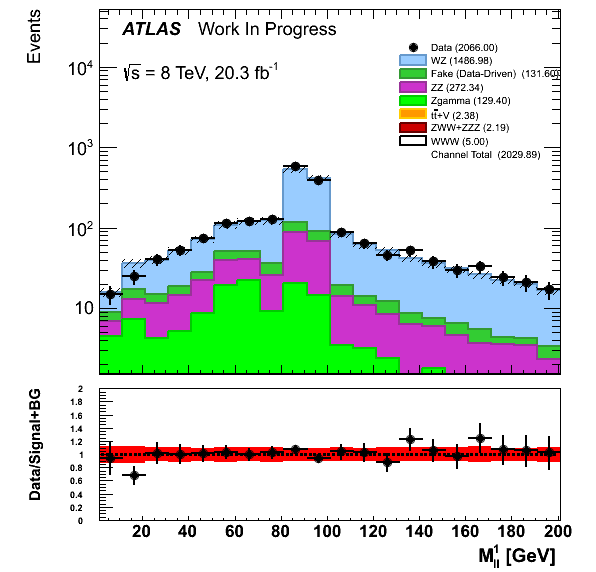
\includegraphics[width=0.495\textwidth]{figures/appendix_signal_selection/Nov24Update_FakeSys_KFacSys_LogY_NoRebin/output/jobs/MxM/DataFull_Rates_May13_FakeRatesExactly2Loose_MuonMxMBJetGt0_ElBJetGt0SubtractPC_MxM/PreselectionNov23_15_2SFOS_ChargeAbs1_BVeto85_physics/weight_all/png/InvariantMassSFOS_histratio.png}
\caption{Plots of the \MET (left) and $m_{\textrm{SFOS}}$ (right) distributions 
in the 1 SFOS (top) and 2 SFOS (bottom) regions after pre-selection
plus the \bee-veto requirement.}
\label{fig:met_zwindow_optimization}
\end{figure}

\begin{figure}[htb]
\centering
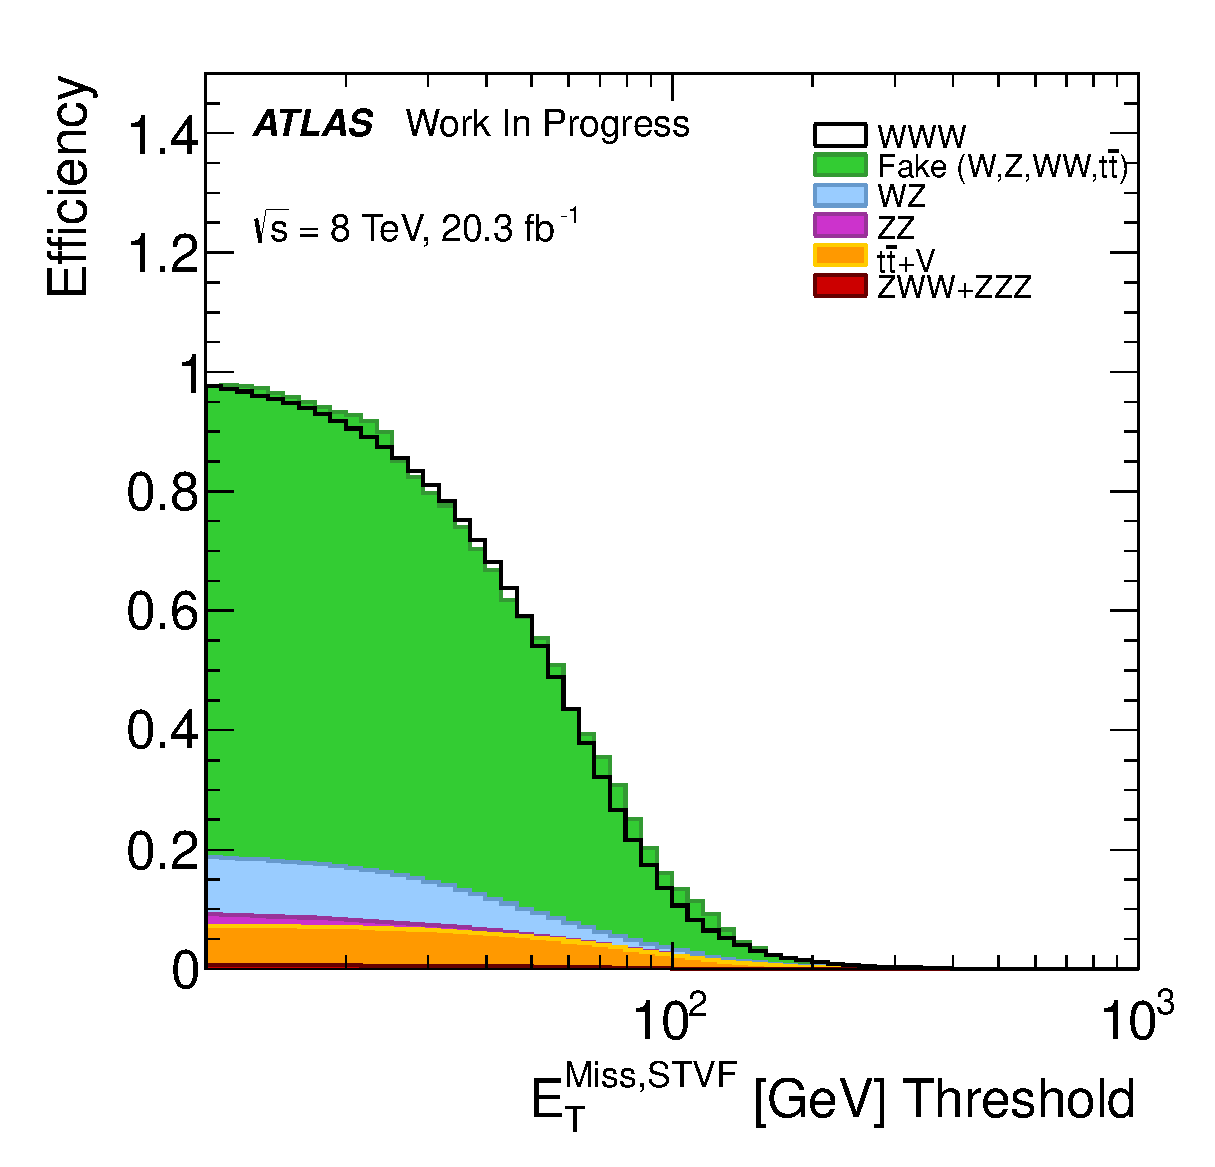
\includegraphics[width=0.495\textwidth]{figures/optimization/SignalRegionsPreselection_0SFOS_Efficiencies/MET_Et_STVF_Cumulative.eps}
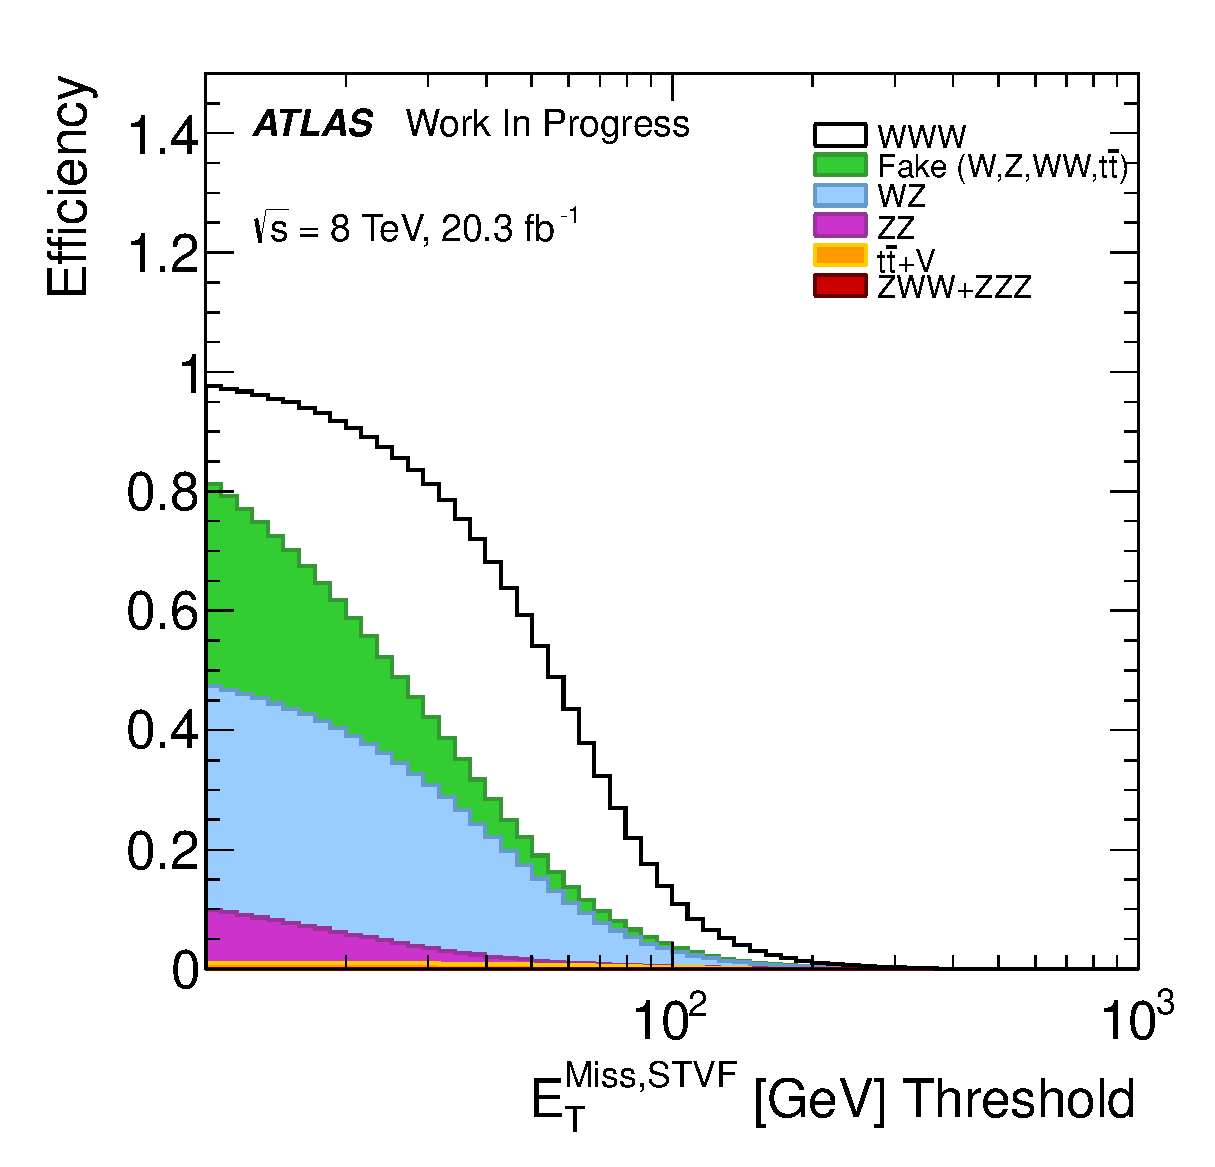
\includegraphics[width=0.495\textwidth]{figures/optimization/SignalRegions_0p5mmZ0_Preselection_Efficiencies/MET_Et_STVF_Cumulative.eps}
\caption{ Signal and background efficiencies for the 
selection, $\MET > X$, as a function of the \MET~selection
threshold, $X$,  in both the 0 SFOS (left) and pre-selection (right) regions.  }
\label{fig:met_eff}
\end{figure}



\begin{figure}[htb]
\centering
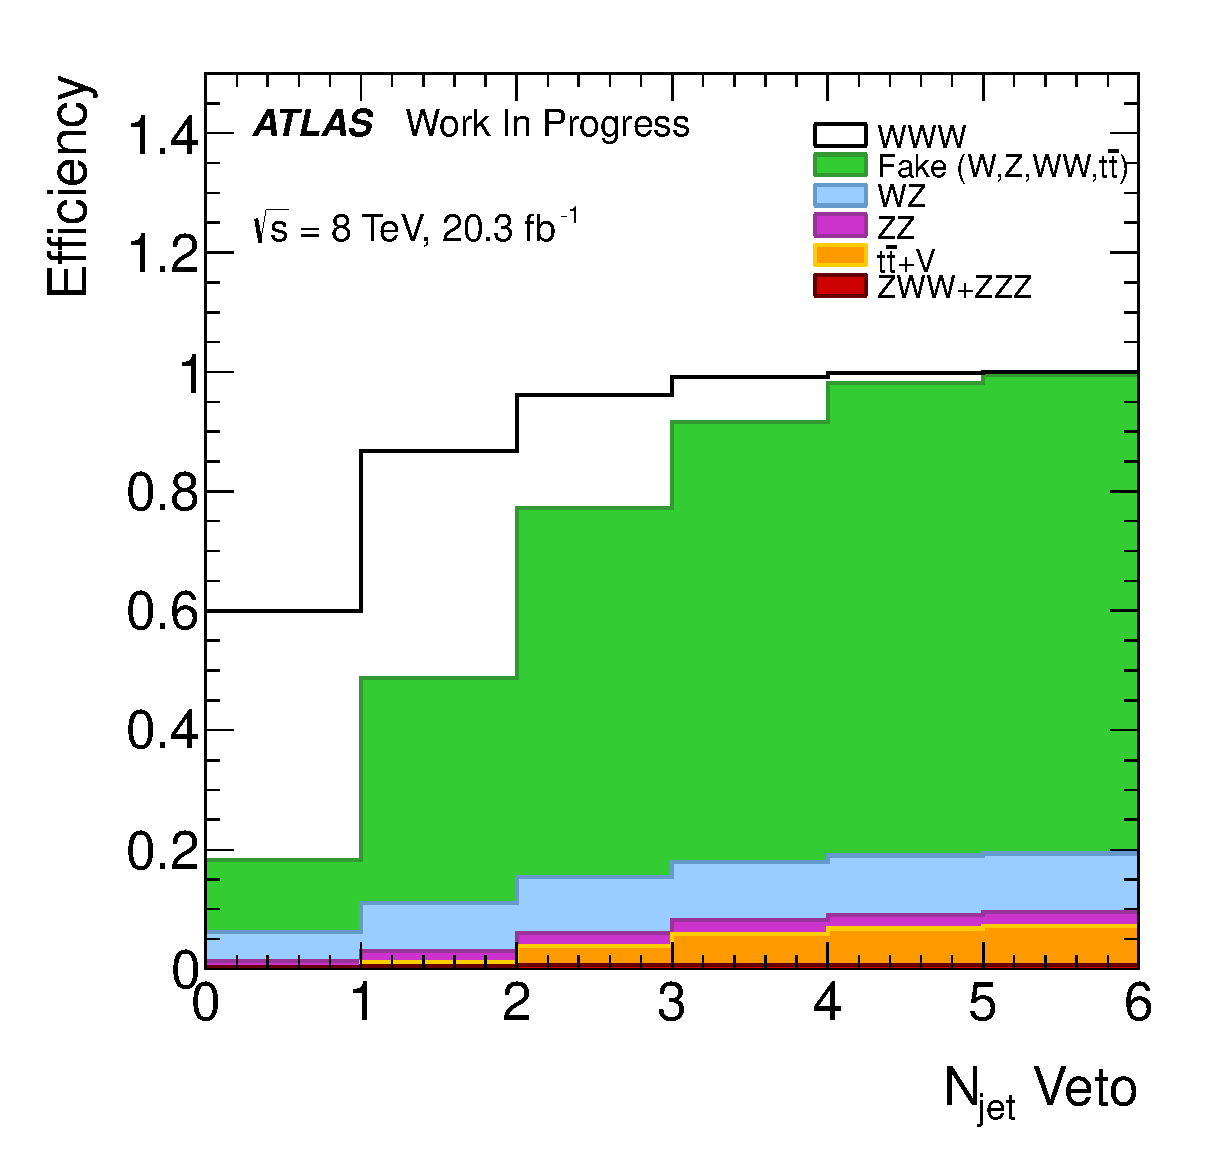
\includegraphics[width=0.495\textwidth]{figures/optimization/SignalRegionsPreselection_0SFOS_Efficiencies/NJets_LeftCumulative.eps}
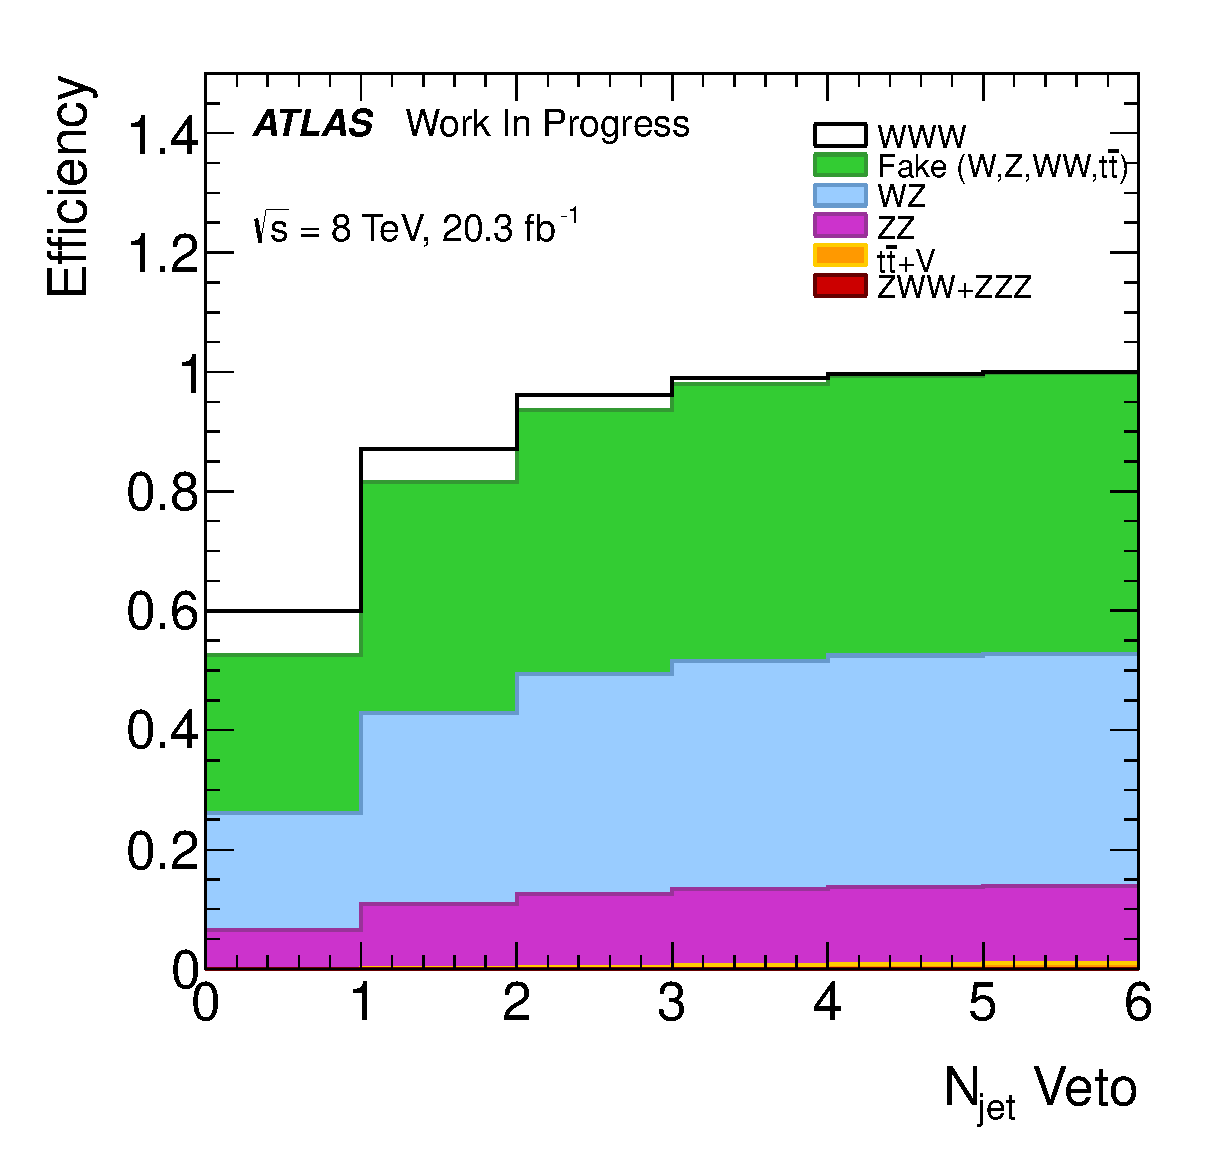
\includegraphics[width=0.495\textwidth]{figures/optimization/SignalRegions_0p5mmZ0_Preselection_Efficiencies/NJets_LeftCumulative.eps}
\caption{ Signal and background efficiencies for the selection,
$\njet \leq X$, as a function of the \njet~selection
threshold, $X$, in both the 0 SFOS (left) and pre-selection (right) regions.  }
\label{fig:njet_eff}
\end{figure}

\begin{figure}[htb]
\centering
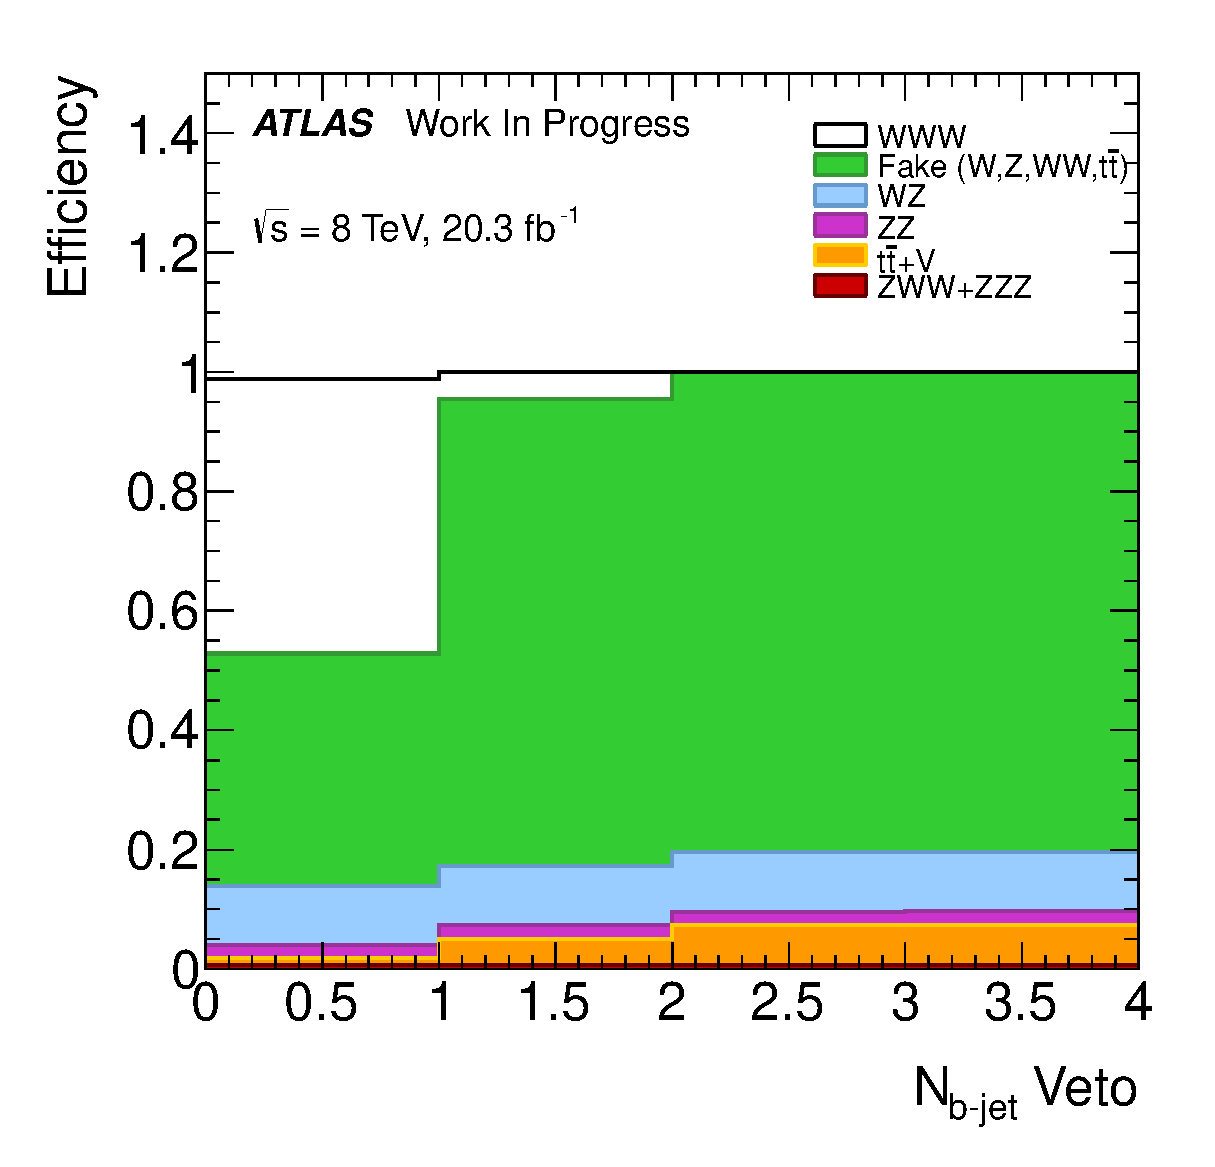
\includegraphics[width=0.495\textwidth]{figures/optimization/SignalRegionsPreselection_0SFOS_Efficiencies/NBTaggedJets_LeftCumulative.eps}
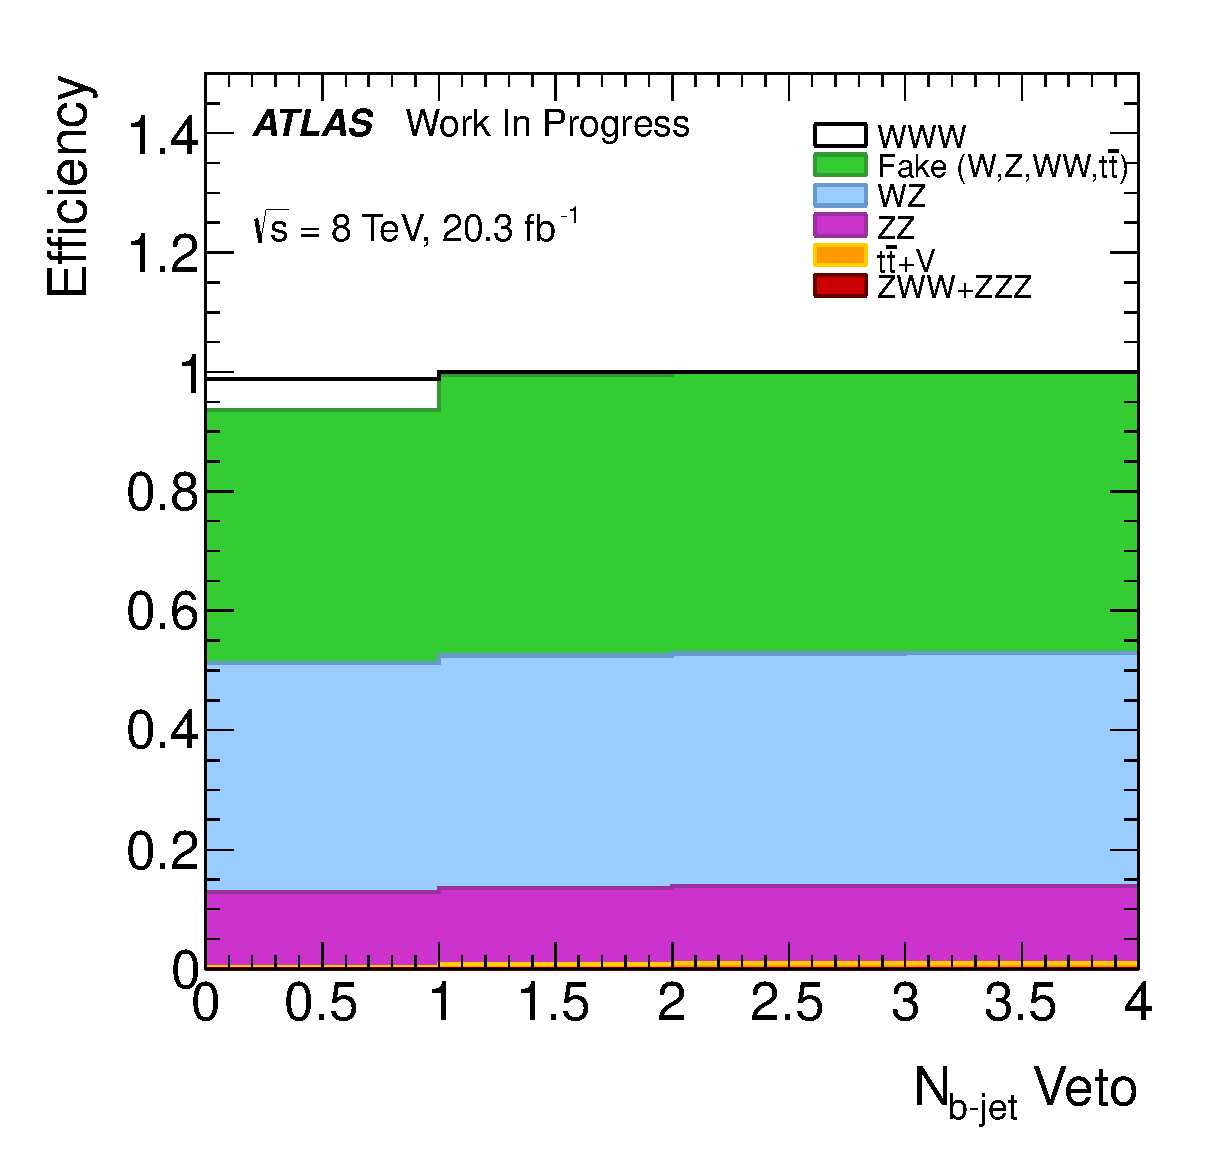
\includegraphics[width=0.495\textwidth]{figures/optimization/SignalRegions_0p5mmZ0_Preselection_Efficiencies/NBTaggedJets_LeftCumulative.eps}
\caption{ Signal and background efficiencies 
for the selection,
$\nbjet \leq X$,
as a function of the \nbjet~selection
threshold, $X$, in both the 0 SFOS (left) and pre-selection (right) regions.  }
\label{fig:nbjet_eff}
\end{figure}


\begin{figure}[htb]
\centering
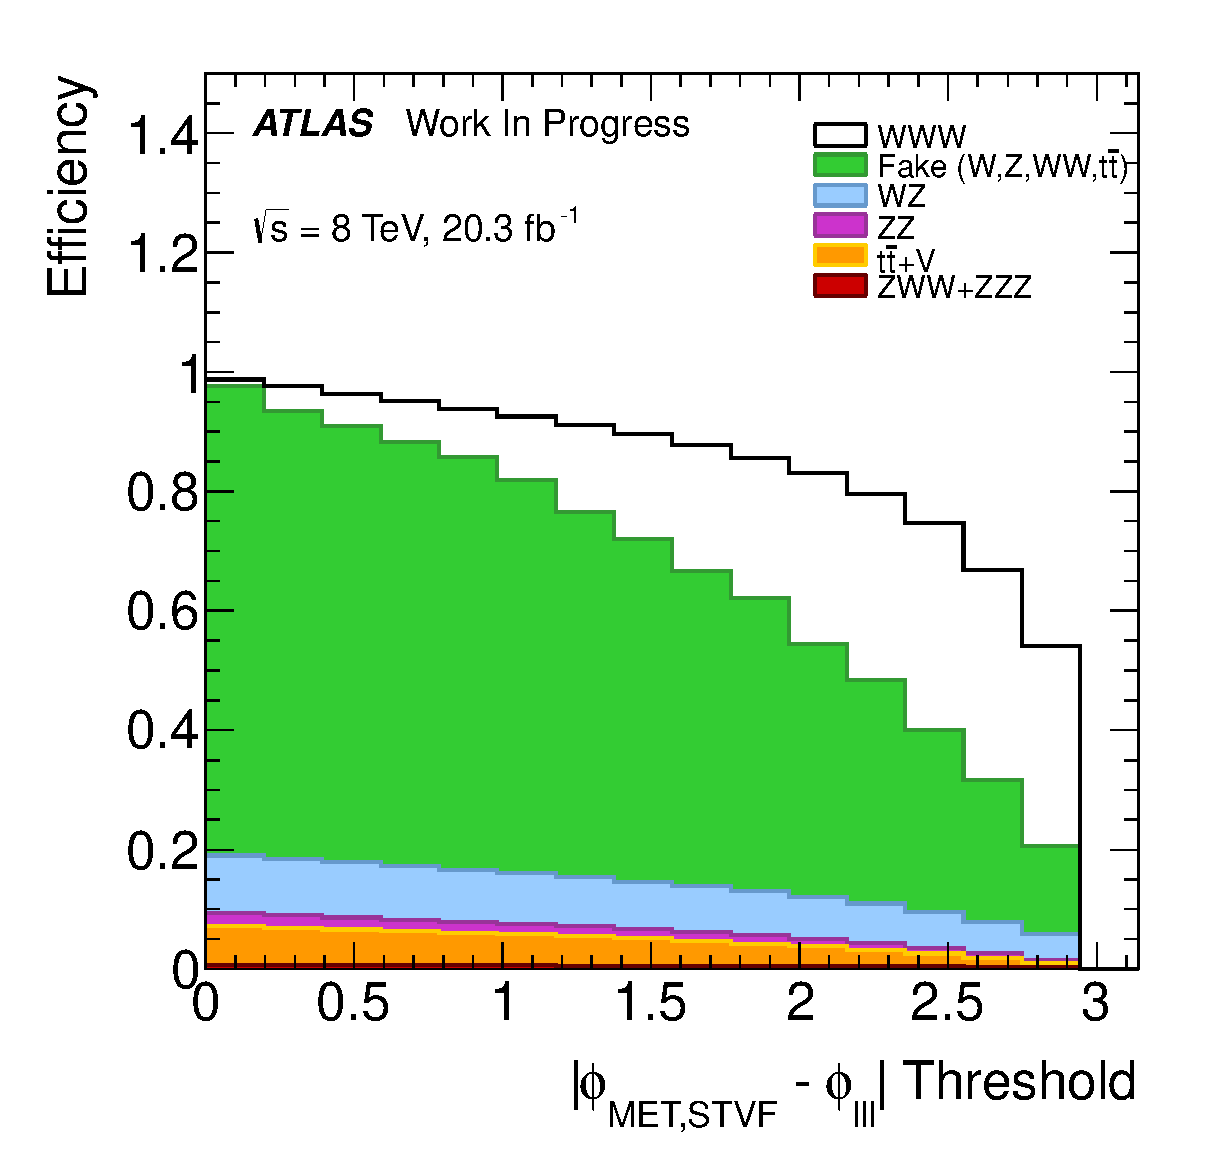
\includegraphics[width=0.495\textwidth]{figures/optimization/SignalRegionsPreselection_0SFOS_Efficiencies/DeltaPhiMETSTVF123_Abs_Cumulative.eps}
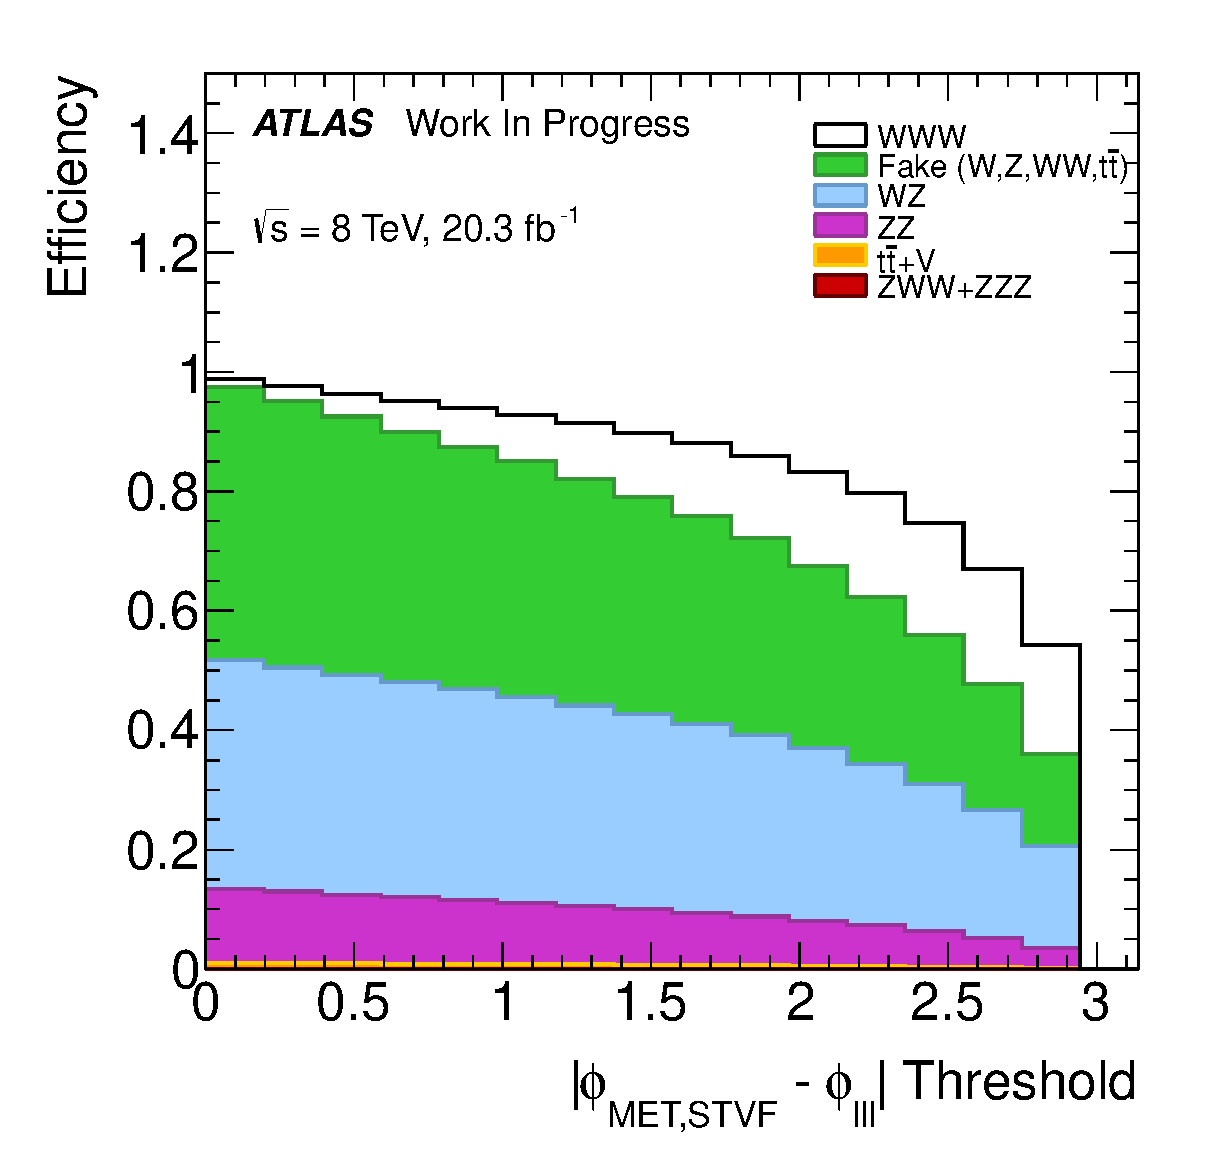
\includegraphics[width=0.495\textwidth]{figures/optimization/SignalRegions_0p5mmZ0_Preselection_Efficiencies/DeltaPhiMETSTVF123_Abs_Cumulative.eps}
\caption{ Signal and background efficiencies 
for the selection,
$|\deltaphi| > X$,
as a function of the \deltaphi~selection
threshold, $X$, in both the 0 SFOS (left) and pre-selection (right) regions.  }
\label{fig:deltaphi_eff}
\end{figure}

\begin{figure}[htb]
\centering
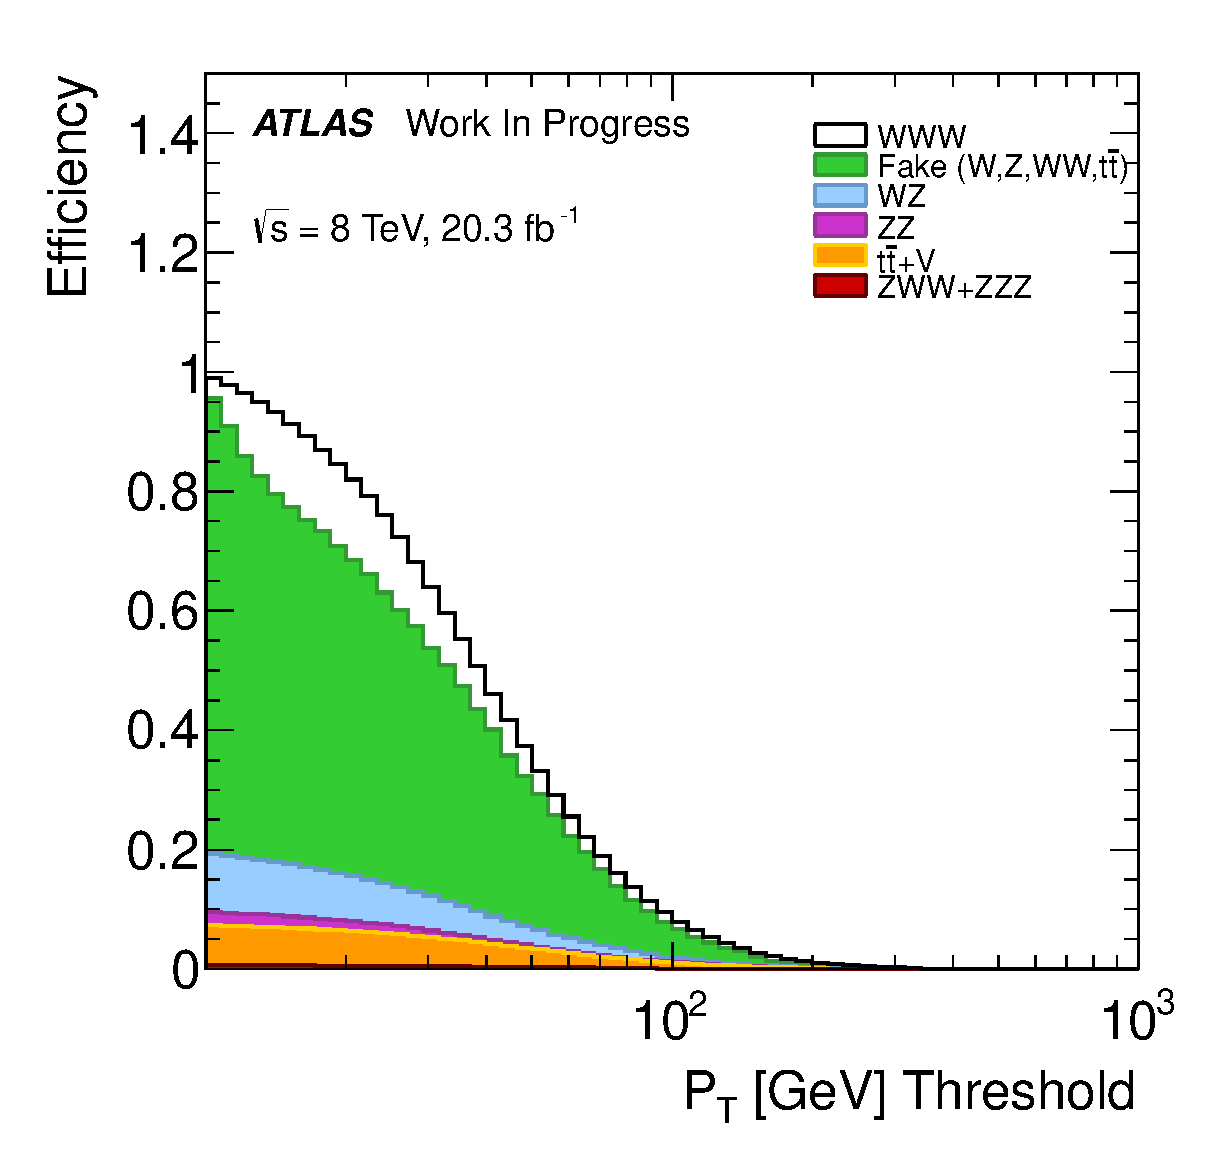
\includegraphics[width=0.495\textwidth]{figures/optimization/SignalRegionsPreselection_0SFOS_Efficiencies/AllLeptonPt_Cumulative.eps}
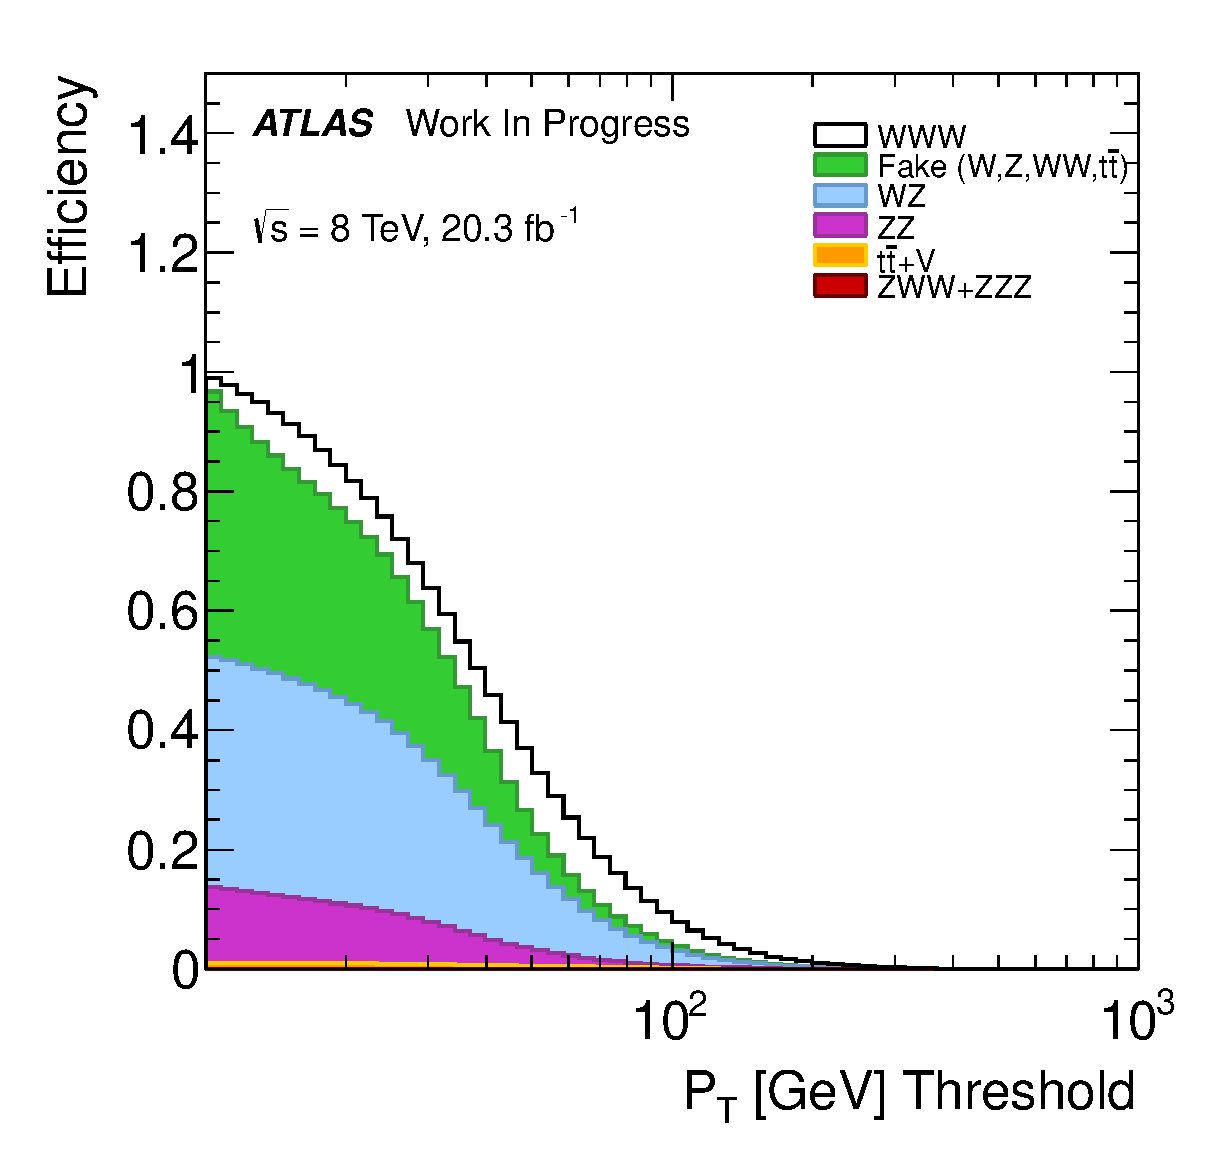
\includegraphics[width=0.495\textwidth]{figures/optimization/SignalRegions_0p5mmZ0_Preselection_Efficiencies/AllLeptonPt_Cumulative.eps}
\caption{ Signal and background efficiencies 
for the selection,
Lepton $\pt > X$,
as a function of the \pt~selection
threshold, $X$, in both the 0 SFOS (left) and pre-selection (right) regions.  }
\label{fig:pt_eff}
\end{figure}

The final selection is presented in \tab\ref{tab:signal_selection}.
Details of the specific cut thresholds that are chosen can be understood
by looking more closely at some of the quantities used as input to 
the optimization. For instance, it is observed that
different \MET~and \z-veto thresholds are chosen for the 1 and 2 SFOS
regions. This can be understood to come from a correlation between
these two quantities due to their ability to isolate the $Z\gamma$
background.
The $Z\gamma$ background shows up in the low-shoulder of the \z-peak
in the $m_{\textrm{SFOS}}$ distribution and at low MET. This can be
seen both for the 1 and 2 SFOS regions in \fig\ref{fig:met_zwindow_optimization}.
As a result, the $Z\gamma$ background can be removed either by tuning 
the \z-mass window used in the veto above, or by removing events with low \met.
Thus, there is some correlation 
between the \z-veto window and the \met~selection threshold. 
In the 1 SFOS region, there is a larger 
contribution from $Z\gamma$ processes than in the 2 SFOS
region.  This process mostly shows up in the low shoulder 
of the \z~ peak. The optimization
prefers removing this $Z\gamma$ contribution by setting an 
asymmetric \z-window in the 1 SFOS
region, with the boundaries being 35~GeV below the \z-pole 
and 20~GeV above and then keeping the \MET~cut a little loose, with a 
threshold of $\MET > 45$~GeV.  In the 2 SFOS region, however,
the $Z\gamma$ contribution is not as prominent and the 
optimization happens to prefer a symmetric
window of $\pm20$~GeV around the \z-pole.  
The looser \z-veto then allows for a tighter
missing $E_{T}$ cut with a threshold of $\MET > 55$~GeV. 


The absence of any cut on the \MET~distribution in the 0 SFOS
region can be better understood by looking at 
the efficiency for selection between 
the signal and the background as a function of the \MET~selection threshold.
This is shown in \fig\ref{fig:met_eff} both after pre-selection
and in the 0 SFOS region.
Clearly, the signal efficiency closely follows the background efficiency
in the 0 SFOS region. Thus, there is no change in the
signal-to-background ratio when cutting on the \MET~distribution
in the 0 SFOS region and thus no improvement in the sensitivity.
On the other hand, there are large shape differences 
between the signal
and background efficiencies at pre-selection, with the 
signal efficiency remaining flatter at low values of the \MET~
threshold. So, from this one would expect a selection
on the \MET~threshold to be useful in the 1 and 2 SFOS
regions which have a similar background composition. 
Indeed, this is what we observe.



The threshold for the jet multiplicity cut 
of $\njet\leq 1$ applied in all signal regions
is also determined from the optimization. One might expect
that a different value for the threshold, such as a complete
veto on the presence of jets, would perform better. 
Indeed, looking at the efficiency for selection on the jet multiplicity
in \fig\ref{fig:njet_eff} does show a much stronger background
rejection when applying a veto in both the pre-selection region
and especially in the 0 SFOS region where there is a larger
contribution from fakes due to hadronic activity.
The signal rejection, however,  of about 40\% observed in both
regions, is prohibitive. Loosening the selection to the nominal
threshold of $\njet \leq 1$ instead preserves 90\% of the signal, 
which is quite precious.  We are still able to remove 
much of the fake background in the 0 SFOS region by vetoing
events with \bee-tagged jets as can be seen in \fig\ref{fig:nbjet_eff}.
%any mention of different operating points
It is possible that using a \bee-tagging operating point
with an even higher \bee-tagging efficiency would further 
improve the sensitivity in the 0 SFOS region.  
The nominal operating point used here, however,  is the highest 
efficiency operating point available.
Clearly, there is no advantage gained from using a looser operating point
as this would only cut less on the background without having an impact
on the signal.





The \deltaphi~distribution for the signal is observed to be more back-to-back
(i.e. closer to $\pi$)
than that for the background. This is especially true in the 0 SFOS
region, as can be seen from the efficiencies plotted 
as a function of the \deltaphi~
selection threshold shown in \fig\ref{fig:deltaphi_eff}.
The selection efficiency for the signal is relatively flat for
most of the range up to about 
a threshold of $|\deltaphi|>2.5$ in both the pre-selection and 0 SFOS
regions.  At this threshold the signal selection efficiency 
is about 80\%.  The optimization prefers a selection
around this range for all signal regions.
The optimization also considered selecting on alternative
definitions of $\Delta\phi$ that only considered one of the three
leptons but this was observed to not offer as strong of a separation
between the signal and background. %figure?


The efficiencies as a function of the lepton \pt~threshold are shown 
in \fig\ref{fig:pt_eff}. 
The signal efficiency is observed to be slightly flatter
than the background efficiency.
The signal efficiency, however,  still falls fairly 
rapidly as a function of the lepton \pt~threshold. 
Thus, a tighter selection on the lepton \pt~is not preferred
by the optimization. We also considered 
applying different \pt~thresholds to the leptons
based on their \pt~order and other criteria, but
this did not show any increased performance.



Finally, we considered other quantities like the 
transverse mass of the \MET~and three lepton system:
\begin{equation}
m_{T}^{lll} = \sqrt{2p_{T}^{lll}\MET(1-\cos(\Delta\varphi(lll,\MET)))},
\end{equation}
as well as vetoes on additional leptons with lower \pt, and various
di-lepton mass selections.  None of these, however, were preferred
by the optimization.

\FloatBarrier
